\chapter{Background}

% Talk about ILP^opl whatever we are using (the latest one)

\section{Answer Set Programming}

Answer Set Programming  \cite{RefWorks:RefID:1-lifschitz2008answer} is a form of declarative programming, with a Prolog-like syntax suitable for solving NP-hard search problems.
However, it is based on a different computation mechanism than Prolog: stable model semantics \cite{RefWorks:RefID:21-fitting1992michael}.
Answer set solver is a program that generates stable models of an answer set program, which are solutions of an answer set program. 
The chosen answer set solver used throughout this project is clingo \cite{RefWorks:RefID:22-clingo}.

This section will briefly highlight the syntax of the answer set programs and the stable model semantics.

\subsection{Syntax}

Here are the types of rules in ASP\footnote{Disjunctive rules also exist, but they are omitted as they are not used in this work.}: 

 1. \emph{normal rule} -> $ h\; :- b_1, b_2, ..., b_n, not\; n_1, not\; n_2, ..., not\; n_o$
 
 2. \emph{hard constraint} -> $:- \; b_1, ..., b_n, not\; n_1, not\; n_2, ..., not\; n_o$
 
 3. \emph{choice rule} -> $lb\{h_1; ..., h_m\}ub\; :- \;  b_1, b_2, ..., b_n, not\; n_1, not\; n_2, ..., not\; n_o$
 
where $lb, ub$ are integers, $n_1,...,n_o$ are atoms and $b_1, ...,b_n$ are either atoms or aggregates.

Aggregates have the following syntax $lb\#agg\{e_1; ...; e_n\}ub$ where $lb, ub$ are ints, $agg$ is an aggregate function (e.g. $sum$) and $e_i$ is an aggregate element.
Additionally, aggregate element has the form  $t_1, ..., t_k : c_1, ..., c_j$ where $t_i$ is a term and $c_i$ is a literal.
 
This syntax is quite expressive. For instance, here are two ways to define a coin falling either on heads or tails.

\subsubsection{Method 1:}
\begin{verbatim}
coin(c1).
heads(C) :- coin(C), not tails(C).
tails(C) :- coin(C), not heads(C).
\end{verbatim}
\subsubsection{Method 2:}
\begin{verbatim}
coin(c1).
1 { heads(C); tails(C) } 1 :- coin(C).
\end{verbatim}

The results of these programs, i.e. the answer sets of the programs, are \{coin(c1), heads(c1)\} and \{coin(c1), tails(c1)\}.
It will be explained how they are computed in the subsequent subsection.

As seen in the example, a program can have multiple answer sets.
So, an additional piece of syntax is defined which evaluates whether some answer set is better than another.
This piece of syntax is referred to as a weak constraint.
It is of the form $:\sim {} b_1,..., b_n.[wt@lev, t1, ..., t_m]$
where $lev$ is an integer, $b_i$ a literal, and $t_i$ term.

\subsection{Semantics}

The Answer Set Programming is based on stable model semantics \cite{RefWorks:RefID:21-fitting1992michael}.

The answer set is defined as follows: 
\emph{Given a program P and a Herbrand interpretation X, X is an \textbf{answer set} of P iff X is a minimal Herbrand model of $RG(P)^X$ (reduct with respect to X).}

To understand the presented definition, one needs to know a few other concepts presented in this subsection.
Here the definitions for those concepts will mainly be explained intuitively rather than formally; for deeper understanding and more formal definitions, please refer to the \emph{Answer Set Programming} book \cite{RefWorks:RefID:23-lifschitz2019answer}. \\

\textbf{Herbrand interpretation} a program is an assignment of every element of the Herbrand base of that program to either true or false. \textbf{Herbrand base} of a program P is a set of all ground atoms that can be made using constants, predicate symbols, and functions of a program P.\\

When a Herbrand interpretation X satisfies all the rules in of a program, X is the \textbf{Herbrand model} of a program. X is also a minimal Herbrand model if there is no smaller subset X', also a Herbrand model.\\

\textbf{Relevant grounding} replaces variables with a program with constants available.
It iteratively fills up the rules by adding every rule whose elements of $body^+$(R) are heads of already included rules. 
The $body^+$ constraint ignores the $not$ atoms. 
For example, take P = \{p(X) :- q(X). q(a).\}. 
The first iteration of relevant grounding would create P' = \{q(a).\} while after the second one P' = \{q(a). p(a) :- q(a).\}\\

The \textbf{reduct of a program} P with respect to X ($P^X$) is a construct used to remove the $not\: c$ terms from a program.
Computing the reduct is done in the following manner. The solver assumes the X is a solution and iterates through every $not\: c$ within P. 
If $c$ is not in X (assumed to be false), then the $not\: c$ term is removed from the rule containing it. 
It essentially removes the need to worry about $not\: c$ since that term is satisfied.
On the other hand, if $c$ is in X, then the entire rule containing $not\: c$ is removed.
There is no need to consider the rule whose body is false since it cannot be satisfied.

Constructing the reduct of a \textbf{choice rule} has an additional step.
It is turned into either normal rules or a constraint.
Given a possible interpretation $X$, the choice rule $lb\{h_1; ..., h_m\}ub\; :- \;  b_1, b_2, ..., b_n, not\; n_1, ..., not\; n_o$ is converted in a following manner:

1. if $ lb \leq |\{h_1; ...; h_m\} \cap X| \leq ub$ then $h_i :- \;  b_1, b_2, ..., b_n, not\; n_1, ..., not\; n_o$ for is created for each $i \in \{1..m\}$

2. Otherwise, a constraint of the form $ :- \;  b_1, b_2, ..., b_n, not\; n_1, not\; n_2, ..., not\; n_o$ 
is created.\\

So, to check whether X is an answer set, one needs to compute a relevant grounding of a program. Then it needs to construct a reduct of that program with respect to X.
From the reduct, one can easily construct a minimal model M by starting from facts and iteratively adding heads of those rules with all body elements already in M.
Finally, if X = M, then X is an answer set.
Note that the head of a \textbf{constraint} is considered to be $\bot$. 
Hence, if the body of a constraint is satisfied, $\bot$ is added to M, so it cannot be equal to X.
In this manner, the constraints eliminate possible answer sets.






% Introduction to stable model semantics and its benefits over other forms of programming.
% Touch upon non-monotonicity. Its non-Turing completeness.

\section{Inductive Logic Programming}

% What is Inductive Logic Programming
Inductive Logic Programming \cite{RefWorks:RefID:42-muggleton1991inductive} is a field at an intersection of machine learning and logic programming.
In most cases, the goal of an inductive learning task is to learn a set of rules (a hypothesis H), which combined with the background knowledge B can entail every positive example while not entailing any negative example. 
Some systems use a weakened version of that statement to allow for noisy examples, such as the newer versions of ILASP \cite{RefWorks:RefID:55-law2018inductive}.

Many ILP systems have been developed over the years, such as Progol5 \cite{RefWorks:RefID:43-muggleton2000theory}, HAIL \cite{RefWorks:RefID:44-ray2003hybrid}, TopLog \cite{RefWorks:RefID:45-muggletontoplog:}, and TAL \cite{RefWorks:RefID:46-corapi2010inductive}.

The chosen system for this project is ILASP \cite{RefWorks:RefID:18-law2020ilasp}, a system that does the inductive learning of the answer sets programs.
Choosing a system that learns ASP is done because the ASP environment can effectively perform non-monotonic reasoning.\\

To understand the ILASP system fully, a few more definitions need to be introduced.

An atom A is \textbf{bravely entailed} if by a logic program P if it is included (true) in at least one answer set of P. 
On the other hand, an atom A is \textbf{cautiously entailed} if it is included (true) in all answer sets of P.

A pair $E = <E^{inc}, E^{exc}>$ (<inclusions, exclusions>) is a partial interpretation of sets of literals.
Answer set X extends E iff set of inclusions is a subset of X ($E^{inc} \subseteq X$) and X is disjoint with exclusions ($E^{exc} \cap A = \emptyset$).


The \textbf{language(inductive) bias} M, is a a pair $<M_h, M_b>$ which is used to construct the \textbf{search space} $S_M$ of a learning task.
The rule of the form  \\$ h \;{:-} b_1, b_2, ..., b_n, not\; n_1, not\; n_2, ..., not\; n_o$ is in $S_M$ iff:
 
 a) $h$ is compatible with $M_h$. This either means that $h$ is an atom compatible with $M_h$, an aggregate $lb\{h_1,.., h_m\}ub$ where each atom $h_i$ is compatible with $M_h$ or $h$ is empty.
 
 b) $b_i$ and $n_i$ are compatible with $M_b$.
 
 c) no variable does not appear in at least one element  of a positive body literal (the rule is safe). \\ 
 
Understanding what compatible refers to in the previous definition is the easiest through the means of an example.

\subsubsection{Inductive bias example}
\begin{verbatim}
#modeh(heads(var(coin))).
#modeh(tails(var(coin))).
#modeha(heads(var(coin))).
#modeha(tails(var(coin))).

#modeb(heads(var(coin))).
#modeb(tails(var(coin))).
#modeb(coin(var(coin))).
#modeb(coin(const(coin))).

#constant(coin, c1).
\end{verbatim}

The example above is a possible definition of the inductive bias for the simple coin problem written in ILASP-compatible syntax.
The \#modeh directive specifies that an atom can occur in the head of the rule. In this case, it defines that $heads(X)$ is compatible with $M_h$.
Similarly, the \#modeha defines that an atom can occur in the aggregate of the rule. Hence, it determines that  $lb\{..., heads(X), ...\}ub$ is a head compatible to $M_h$.
The \#modeb syntax defines that an atom can occur in the body either as a positive or negative atom.
Finally, the \#constant defines constants that can replace const functions.

Let $S_M$ be the search space constructed from the language bias M, B background knowledge, $E^+$/$E^-$ set of positive/negative examples, T = $<B, S_M, E^+, E^->$ is the \textbf{learning from answer set task} \cite{RefWorks:RefID:47-law2014inductive}.
The hypothesis H is a set of inductive solution iff:

1. It is a subset of search space $S_M$.

2. For every negative example $e^-$, there is no answer set A of the program $B \cap H$ which extends that example.

3. For every positive example $e^+$, there is an answer set A of the program $B \cap H$ which extends it.
\\

Notice that the positive examples are bravely entailed while the negative are cautiously entailed.\\

\subsubsection{Examples in ILASP}
\label{examples-in-ilasp}

\begin{verbatim}
#pos(
{heads(c1)},
{tails(c1)},
{coin(c1).}
).

#neg(
{tails(c2), heads(c2)},
{},
{coin(c2).}
).
\end{verbatim}

The shown piece of code is a simple definition of examples in ILASP. 
Both positive and negative take either 2 or 3 parameters. The first two are the set of inclusions $E^{inc}$ and the set of exclusions $E^{exc}$.
The third optional parameter is the context $C_e$ of an example.
The context of an example, $C_e$ is a set of rules and facts that are only relevant when explaining the example $e$.
With this parameter, the agent tries to find hypothesis H such that an answer set of $B \cap H \cap C_e$ extends $e$ (for positive $e$).
The analogue holds for negative examples. 
A formal definition of the Context-dependent Learning from Ordered Answer Sets framework can be found in work by Broda et al., \cite{RefWorks:RefID:56-broda2016iterative} which introduced context-dependent examples to ILASP. \\

FastLAS \cite{RefWorks:RefID:19-law2020fastlas:}, a much faster alternative to ILASP, has been developed recently.
Unfortunately, to get to the desired level of scale, the system operates with certain constraints which are too restrictive for this project.
For example, the programs constructed will generate at most one answer set.

% Link to Tutorials for FastLas, ILASP

\section{Natural Language Processing}

The critical requirement of this project is to extract syntactic concept sentences from the text corpus.
This section has a brief overview of the techniques applied to make the concept extraction possible.

The techniques presented in the following section are implemented by a popular library \emph{spacy} \cite{RefWorks:RefID:24-spacy} which has been utilised in this project. 
The language model currently used throughout the project is \emph{en\_wb\_gl\_lg}, but a more performant option may replace it after further investigation.

\subsection{Preprocessing Techniques}

\textbf{Tokenisation} separates the given text into smaller units named \emph{tokens}. 
It is common to split English text into words as tokens, as they carry meaning and are easy to extract.
The \emph{spacy} library implements such behaviour with it additionally separating punctuation into separate tokens.\\

\textbf{Sentence splitting} is a similar problem as tokenisation. It splits a text corpus into sentences before they are processed individually. \\

% TODO think of better %
\textbf{Word Normalisation} replaces words with a consistent form which greatly simplifies recognition of identical words.
Some of the reasons different forms of words arise are capitalisation (Cat, cat -> cat), acronyms (U.S.A/USA/U S A -> USA) and spelling variants (chequebook/cheque book -> cheque book). 
Most of the words can be modified by applying rule-based modifications, but there needs to be special handling of some words which have double meaning such as \emph{Turkey} (bird/country). \\


% tag spacy PoS 
\textbf{Part-of-speech tagging} attempts to determine which tag does a word have in the sentence.
The problem is much more complicated than the ones previously described as the part of speech can often be dependent on the meaning of the word in a sentence.
For example, the sentence \emph{I play the main character in a play} highlights how word \emph{play} can have two identically written words that can have different meanings and parts of speech.
The first occurrence of \emph{play} is a verb, and the second is a \emph{noun}.

The spacy library uses neural networks and statistical models to determine which tokens the library should assign which POS tag \cite{RefWorks:RefID:25-spacy}.
The classifier which spacy uses has a very high accuracy for the English language, with accuracy between 97-98\% depending on the model \cite{RefWorks:RefID:26-spacy}.


% http://nlpprogress.com/english/dependency_parsing.html - tracks state of the art

\subsection{Parsing}

\subsubsection{Dependency Parsing}

Dependency Parsing is a form of parsing that attempts to determine words' dependency within a sentence \cite{RefWorks:RefID:28-jurafsky2014speech}.

The resulting structure obtained is a dependency parse tree.
An example of a dependency parse tree can be seen in \ref{dependency-graph}.
This structure enables determining which purpose does a word serve in a sentence.
To illustrate why determining what purpose a word serves in a sentence may be helpful, here is a predicate/subject refresher:
\emph{The subject is a person/object who/what the sentence is about, while the predicate tells what the subject is or what it is doing} \cite{RefWorks:RefID:27-subject}.
From this definition, it is clear that one can easily extract an actor in a sentence if they know what it is doing.
The dependencies produced by the \emph{spacy} dependency parser are more precise as they follow \hyperlink{https://univesaldependencies.org}{Universal Dependencies}.
For instance, those dependencies distinguish between nominal and clausal subjects.
Please refer to the \hyperlink{https://univesaldependencies.org}{Universal Dependencies} to see a complete list of the dependencies available if needed. 

% How does it work? Maybe describe Mniri et al approach if lacking content

% What is the performance.
To evaluate the performance of a dependency parser, one uses labelled attachment score (LAS) and unlabelled attachment score (UAS) accuracy \cite{RefWorks:RefID:28-jurafsky2014speech}.
The former validates how well a word is assigned to its head and whether a correct dependency relation is assigned.
The latter score checks whether the head is assigned correctly.
Spacy's dependency parsing system slightly trails behind the state of the art approaches at the moment, with its UAS and LAS being at 95.1\% and 93.7\%, respectively. 
Mniri et al. \cite{RefWorks:RefID:29-mrini2019rethinking} developed the current state of the art model, with UAS/LAS scores at 97.4\% and 96.3\%.

\begin{figure}[h]
\caption{Dependency graph of \emph{The fielder caught the ball.}}
\centering
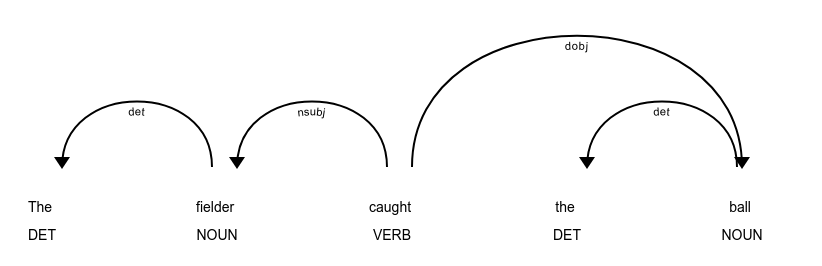
\includegraphics[width=\textwidth]{background/dependency_graph.png}
\label{dependency-graph}
\end{figure}

\subsubsection{Constituency Parsing}

Constituency Parsing is a form of syntactic parsing which assigns a structure to a sentence created by a context-free grammar \cite{RefWorks:RefID:28-jurafsky2014speech}.
This approach aims to group words into constituents, a group of words that behave as a single unit.
For example, one may group a sequence of words surrounding a noun into a noun phrase such as \emph{the Imperial students}.
Words grouped into constituents can be used as an intermediate form for semantic analysis and checking whether a sentence is grammatically correct.
In the context of this project, it will be utilised as a part of atomic sentence extraction.


The resulting structure produced by constituency parsing is a parse tree. 
An example of a tree parsed by a constituency parser can be seen in \ref{constituency-graph}.

\begin{figure}[h]
% https://parser.kitaev.io/
% INSERT https://spacy.io/universe/project/self-attentive-parser
% TODO find where labels are defined.
\caption{Parse tree of \emph{The fielder caught the ball.} as generated by spacy Berkley Neural Parser.}
\centering
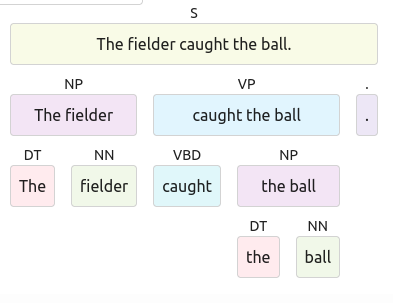
\includegraphics[width=0.8\textwidth]{background/constituency parse.png}
\label{constituency-graph}
\end{figure}

% How is it done if need more content?

% \section{Other Relevant Machine Learning Topics}
% 
% TODO
% 
% \subsection{Video Processing}
% 
% \subsubsection{Convolutional Neural Networks}
% 
% % Check those from their papers.
% 
% % Check more stuff from computer vision.
% 
% \subsubsection{Feature Extractors}
% 
% \subsection{Attention}






